%                                                                 aa.dem
% AA vers. 9.1, LaTeX class for Astronomy & Astrophysics
% demonstration file
%                                                       (c) EDP Sciences
%-----------------------------------------------------------------------
%
%\documentclass[referee]{aa} % for a referee version
%\documentclass[onecolumn]{aa} % for a paper on 1 column  
%\documentclass[longauth]{aa} % for the long lists of affiliations 
%\documentclass[letter]{aa} % for the letters 
%\documentclass[bibyear]{aa} % if the references are not structured 
%                              according to the author-year natbib style

%
\documentclass{aa}  

%
\usepackage{graphicx}
%%%%%%%%%%%%%%%%%%%%%%%%%%%%%%%%%%%%%%%%
\usepackage{txfonts}
%%%%%%%%%%%%%%%%%%%%%%%%%%%%%%%%%%%%%%%%
%\usepackage[options]{hyperref}
% To add links in your PDF file, use the package "hyperref"
% with options according to your LaTeX or PDFLaTeX drivers.
%
\begin{document} 


   \title{The variability  of Betelgeuse explained by surface convection}


    \author{{ Q.~Pilate}\inst{1},{ A.~L{\'o}pez Ariste}\inst{1},{ A.~Lavail}\inst{1},{ Ph. Mathias}\inst{1} }

   \institute{IRAP, Universit\'e de Toulouse, CNRS, CNES, UPS.  14, Av. E. Belin. 31400 Toulouse, France 
             }

   \date{Received ...; accepted ...}

% \abstract{}{}{}{}{} 
% 5 {} token are mandatory
 
  \abstract


   \keywords{
               }

   \maketitle
%
%-------------------------------------------------------------------

\section{Introduction}

Betelgeuse is a prototypical red supergiant (RSG) known to be a semi-regular variable. Several periods can be found in the 
literature usually clustered around the so-called long secondary period (LSP) of 2000 days and other more or less well defined 
periods around 400 and 200 days. Such periods are often linked to radial pulsation modes,   and have been used to model 
the caracteristics of the resonant cavity, hence the size of the star and eventually its evolutionary stage \cite{XXX}.

At the end of 2019, Betelgeuse suffered a sudden and dramatic loss of brightness \cite{}, particularly in the blue colors. 
\cite{Miguel} has demonstrated that such event was due to the emission by the star of a cloud of dust near to the line of sight of 
Earth. In this event it was clear that a change in brightness was not due to any kind of pulsation but to a change on the 
brightness distribution over the stellar disk due to the presence of large quantities of dust. While this may be seen as 
a singular event, it brings up the question whether all changes in brightness cannot be due to similar changes in the brightness 
distribution over the disk. 

Betelgeuse is known to present large convective cells with life times in the order of one to two years and measurable changes 
in the span of one week. Bright convection cells near disk center will increase the integrated brightness of the star when 
compared with other situations where such cells are found near the edges. So even without calling for the formation of 
dust or other changes in opacity, one may argue that the simple convective patterns of the star may create a variability. Such 
variability could be expected to be random, but will present quasi-periodicities related to the typical time scales of the 
convective patterns. 

Since the end of the Great Dimming event, Betelgeuse has continue its random variation of brightness. But the classical periods 
of variation cited above are not visible any more. This may be due to simply the short span of time, that does not afford for 
the peaks to appear prominently in the variability spectra. But it has been sufficient to bring up that other explanation of the variability
in terms  of convective patterns. In order to address this question we seek for the typical periods of 1000, 400 and 200 days in  
observational proxies related to the convective activite but unrelated to pulsations nor directly linked to brightness?

Linear polarization in the atomic lines of the spectra of Betelgeuse, discovered by \cite{auriere_discovery_2016}, has been interpreted as the joint action of 
two mechanisms. First the depolarization of the continuum by atoms which absorb linearly polarized light and re-emit unpolarized light, the 
continuum photons being polarized by Rayleigh scattering. This depolarization produces signals with an azimuth symmetry over the disk that 
would  cancel out the net linear polarization on a homogeneous disk. Thus it must be combined with an inhomogenous disk to produce the net linear polarization 
signal observed. This interpretation suggested the possibility of mapping those brightness inhomogeneities. This has been done by \cite{lopez_ariste_convective_2018} 
even producing 3-dimensional images of the atmosphere of Betelgeuse \citep{lopez_ariste_three-dimensional_2022} when taking advantage of the different height of formation of 
different lines in the spectrum of Betelgeuse. The images produced compare very well with cotemporaneous images made with interferometric 
techniques and show clear convective patterns. Linear polarization in the atomic lines is therefore a proxy of convection, unrelated to radial 
pulsations but linked to the brightness inhomogeneities due to the convective patterns in Betelgeuse. If one can find the aforementioned periods 
in linear polarization, we must conclude that these periods are related to the convective activity which originates those linear polarization 
and unrelated to any radial pulsation phenomena.




Betelgeuse is a red super giant star which has been observed by many astronomers for centuries. This star is known as a 
semi variable star. In the literature, the variability of the light curve of Betelgeuse is mainly explained by pulsation of 
the atmosphere. The most common periods found in Betelgeuse are the long secondary period (LSP) which is around $2000$ days 
and there are few known overtones such as $400$ days or $200$ days. Since the great dimming between the end of 2019 and 
beginning of 2020, those periods have changed. In this article, we attempt to recover the different periods of Betelgeuse 
using surface convection. The brightness of Betelgeuse is linked to the giant convective cells present at the surface. Hence, 
the light curve will be affected by the size and the number of convective cells at the surface and also by the timescale on 
those convective cells live. To explain to variability of Betelgeuse, we used the polarimetric data from the telescope Bernard 
Lyot, which observed Betelgeuse over a decade almost weekly. The linear polarization in Betelgeuse is associated to brightness 
inomogeneities at the surface of the star, due to huge convective cells at the surface. From the linear polarization signal, 
we were able to produce images of Betelgeuse. From the variability of the linear polarization and the intensity signal, we 
attempted to recover the variability of Betelgeuse. We also tried to recover the variability using the images produced by 
polarimetry. The photo-center displacement is affected by the size, number and timescale of convective cells. Using our 
images, we followed the displacement of the photo-center of Betelgeuse over 10 years to recover the variability of 
Betelgeuse. 

\section{Method: Searching for periodicities in the polarization spectra of Betelgeuse}

Betelgeuse has been observed for the last 13 years with Narval and Neo-Narval at the Telescope Bernard Lyot. These instruments measure the polarization 
over the visible spectra of Betelgeuese (390-1000 nm) with high spectral resolution (R=65000) and high polarimetric sensitivity. Despite 
this sensitivity, the signal-to-noise ratios are not sufficient to measure the weak polarization signals in the individual atomic lines of the 
spectrum. These amplitudes are today known to be of the order of $10^{-4}$ times the continuum intensity, and only excepcionnaly do they 
reach amplitudes of $10^{-3}$ the continuum. In these exceptional observations, enough photons can be accumulated per spectral bin to 
see the linear polarization signal above noise \citep{auriere_discovery_2016}. Most commonly, the amplitudes of linear polarization are below noise levels. In those 
occassions we have to add up the signals of thousands of lines to reduce the noise and increase the signal-to-noise ratios. This line addition 
is done through a technique called Least-Squares Deconvolution (LSD) \citep{donati_spectropolarimetric_1997} and assumes that the 
linear polarization signal is similar 
in all spectral lines up to scale factors in the sampling and amplitude. This technique has been successfully used in the past to measure 
magnetic field distributions over stellar surfaces and it is now used to produce images of the brightness distributions in the photosphere 
of Betelgeuse and other red supergiants as cited in the Introduction. 

In this work we shall look into the signals produced through these line-addition techniques, and which produce a pseudo-spectral line in intensity 
and linear polarization which does not belong to any atomic species in particular but to an average of all of them present and emitting in the 
photosphere of Betelgeuse. These signals carry the coherent signals present in the photospheric lines, but the particularities of this or 
that spectral line are erased. All these data has been presented before by \cite{auriere_discovery_2016}, \cite{mathias_evolution_2018} and 
\cite{lopez_ariste_three-dimensional_2022}, which also give details on observing times and conditions as well as more detailed description 
on the data reduction \footnote[1]{Beyond a 2-year proprietary embargo, and up to technical issues, all these data is available through 
PolarBase (http://polarbase.irap.omp.eu/).}



\subsection{Lomb-Scargle periodogram}

Trying to find periods in an astrophysical context can be difficult due to the unevenly spaced observed data. To overcome this issue, 
we used the Lomb-Scargle (LS) periodogram \citep{Lomb1976,Scargle1982}. For a given set of data, it fits a sinusoid function using least-squares at each 
frequency between the first and the last observation. The better the fit, the higher the power attributed to the given frequency. Since Betelgeuse has 
been observed by the Télescope Bennard Lyot at pic du midi since 2013, we have ten years of data. Betelgeuse was observed every two or three weeks by 
the spectropolarimeters Narval and Neo-Narval, except during summer. From all these data, we can compute least-squared 
deconvolution (LSD) \citep{Donati1997} profile of Stokes I, U and Q. The linear polarization present in Betelgeuse is attributed to brightness 
inhomogeneities, which are due to the convective cells present at the surface \citep{LopezAriste2018}. To recover variability of Betelgeuse, 
we computed the LS periodogram at each wavelength of the LSD profile, between -25 km/s and 80 km/s. We choose those velocity to span the entire 
signal present in the LSD profile. In the work of \cite{LopezAriste2018}, the most blueshifted signal was present at -20 km/s, 
corresponding to the maximal velocity of the rising plasma. The most redshifted signal was $\sim$ 40 km/s. This velocity corresponds 
to the velocity of the star in our reference frame \citep{LopezAriste2018}. 


\subsection{Before and after the dimming}

At the beginning of 2020, Betelgeuse reached a historical minimum in its luminosity, called the great dimming \citep{Guinan2020}. 
From interferometric data, we know that this event was caused by a cloud of gas in front of the line of sight \citep{Montargès2021}. 
Interferometric images show a huge drop in luminosity in the southern hemisphere of Betelgeuse, leading to this dimming. Interestingly, 
it has been shown by \cite{jadlovsky2022} that the periodicity of Betelgeuse has changed before and after the dimming. Using the light curve from AAVSO, 
the authors showed that before the dimming, the dominant period of Betelgeuse was around 400 days. However, after the dimming, this period has changed and 
is now shorter, around 200 days. It means that, after the dimming, there was a change in the behaviour of the atmosphere of Betelgeuse: the period is now
shorter than before the dimming. Our analysis is based on this change of periodicity. By computing the Lomb-Scargle periodogram for each frequency 
in the LSD profile, we expect to find periodicities around the LSP, but also on the 400 days and 200 days period. However, we expect a change
in the periodicity after the dimming. This would lead to a decrease in the Lomb-Scargle power. 
Figure \ref{LS intensity},\ref{LS Q},\ref{LS U} and \ref{LS linear polarization} show the Lomb-Scargle periodogram of the LSD profile of respectively 
the intensity, stokes Q, stokes U and the linear polarization. The abscissa is the frequency, while the ordinate is the heliocentric radial velocity. 
For each figure, the upper panel is the LS periodogram with data taken before the great dimming of Betelgeuse, that is from 2013 to 2019. 
The lower panel is the LS periodogram for the data before and after the dimming: from 2013 to 2023. The white dashed lines represent the different 
periods found in the literature: the LSP at 2000 days, the fondamental pressure mode at 400 days and its first overtone at 200 days. The Lomb-Scargle 
power is normalised. The colorbar indicates the quality of the fit: red areas correspond to good fits from the LS periodogram, those areas are good 
candidates for periodicities. 

\begin{figure*}[!h]
    \centering
    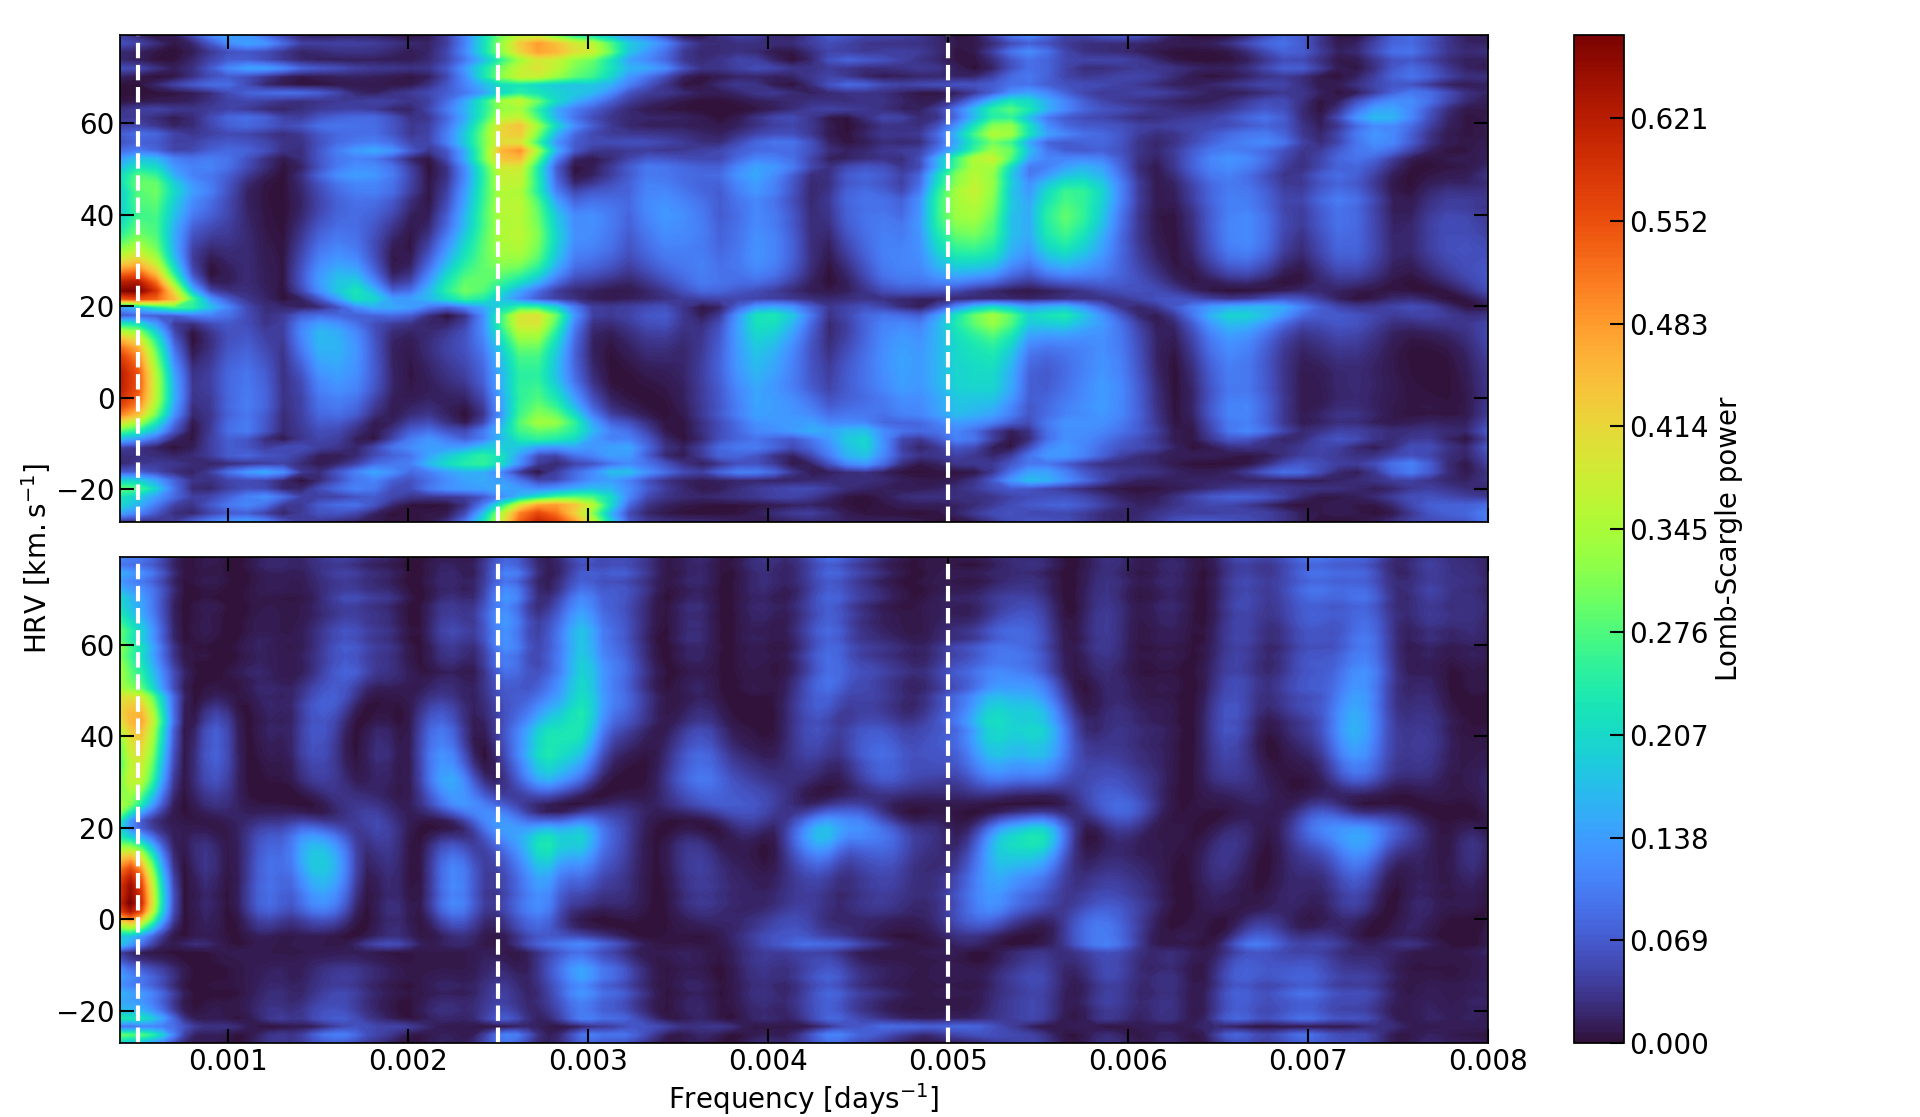
\includegraphics[width=\textwidth]{Lomb-Scargle Intensity.png}
    \caption{Lomb-Scargle periodogram of the LSD profile of the intensity. The upper pannel is the LS periodogram for data before the great dimming. The lower panel is periodogram after the dimming. The ordinate refers to the velocity in the heliocentric radial velocity in km/s. The abscissa is the period in $\mathrm{days^{-1}}$. The three white dashed lines represent respectively (from left to right) the LSP at 2000 days, the 400 days period and its first overtone at 200 days. The Lomb-Scargle power refers to the quality of period found. }
    \label{LS intensity}
\end{figure*}

\begin{figure*}[!h]
    \centering
    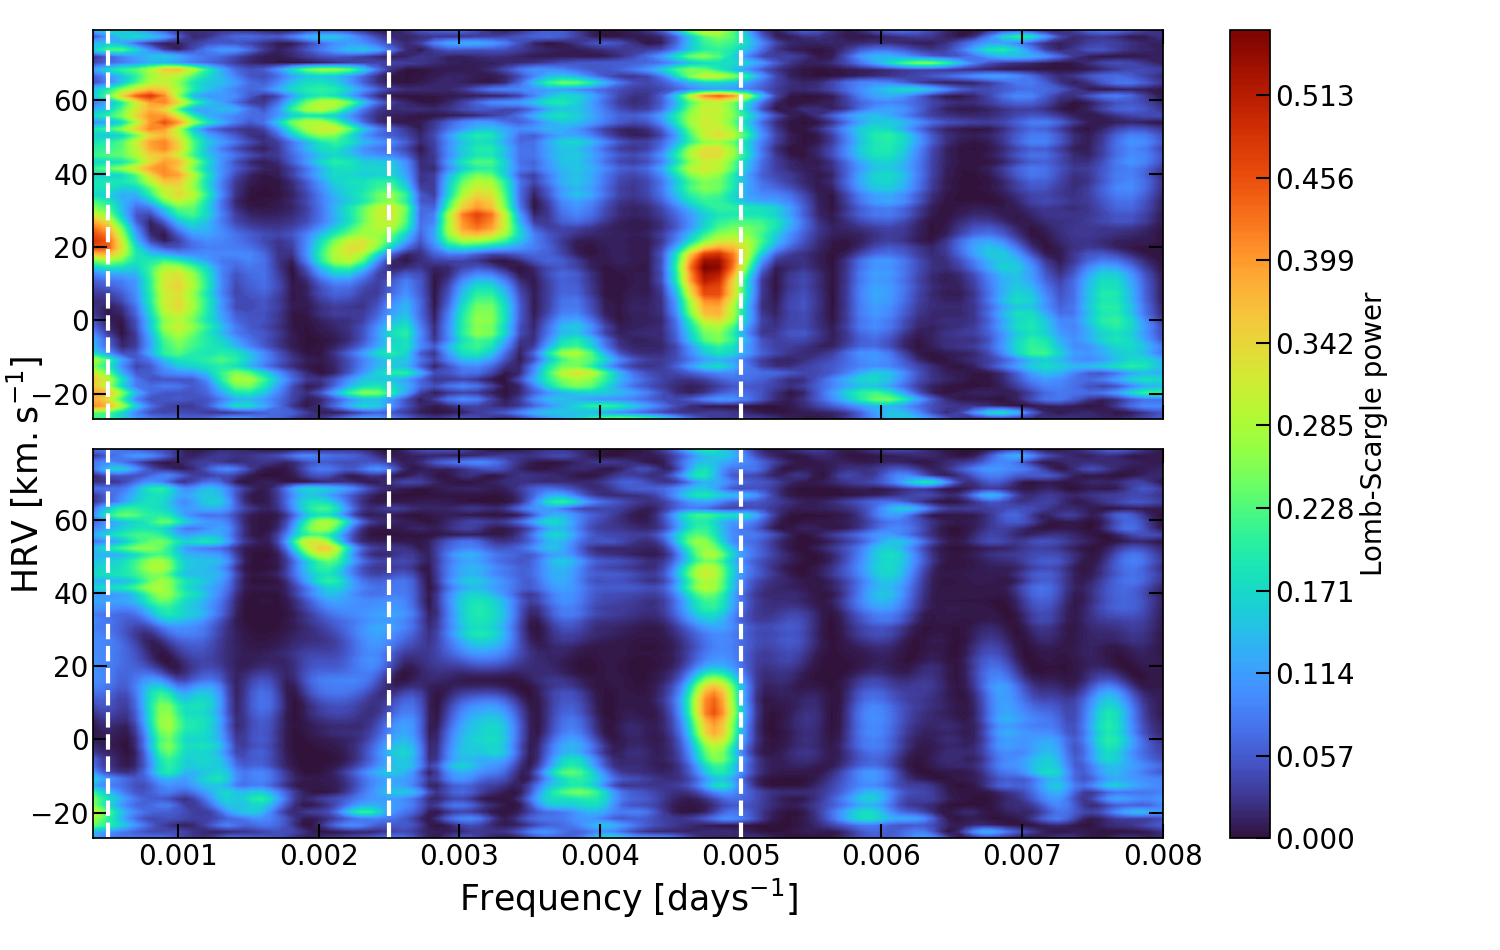
\includegraphics[width=\textwidth]{Lomb-Scargle Stokes Q.png}
    \caption{Same as figure \ref{LS intensity} but for stokes Q. }
    \label{LS Q}
\end{figure*}

\begin{figure*}[!h]
    \centering
    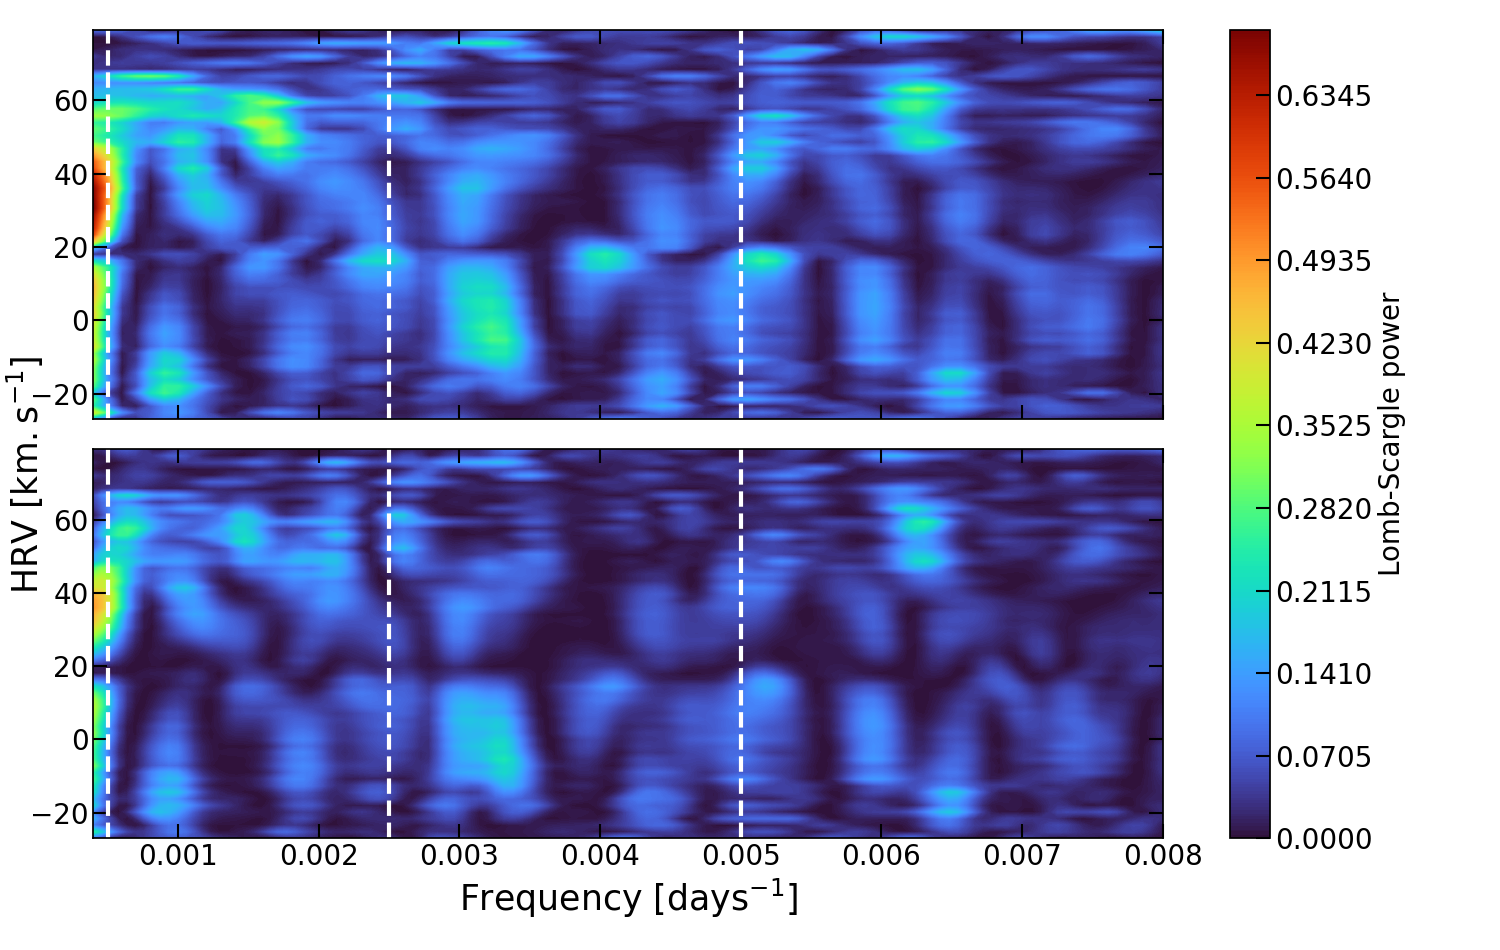
\includegraphics[width=\textwidth]{Lomb-Scargle Stokes U.png}
    \caption{Same as figure \ref{LS intensity}, but for stokes U.}
    \label{LS U}
\end{figure*}


\begin{figure*}[!h]
    \centering
    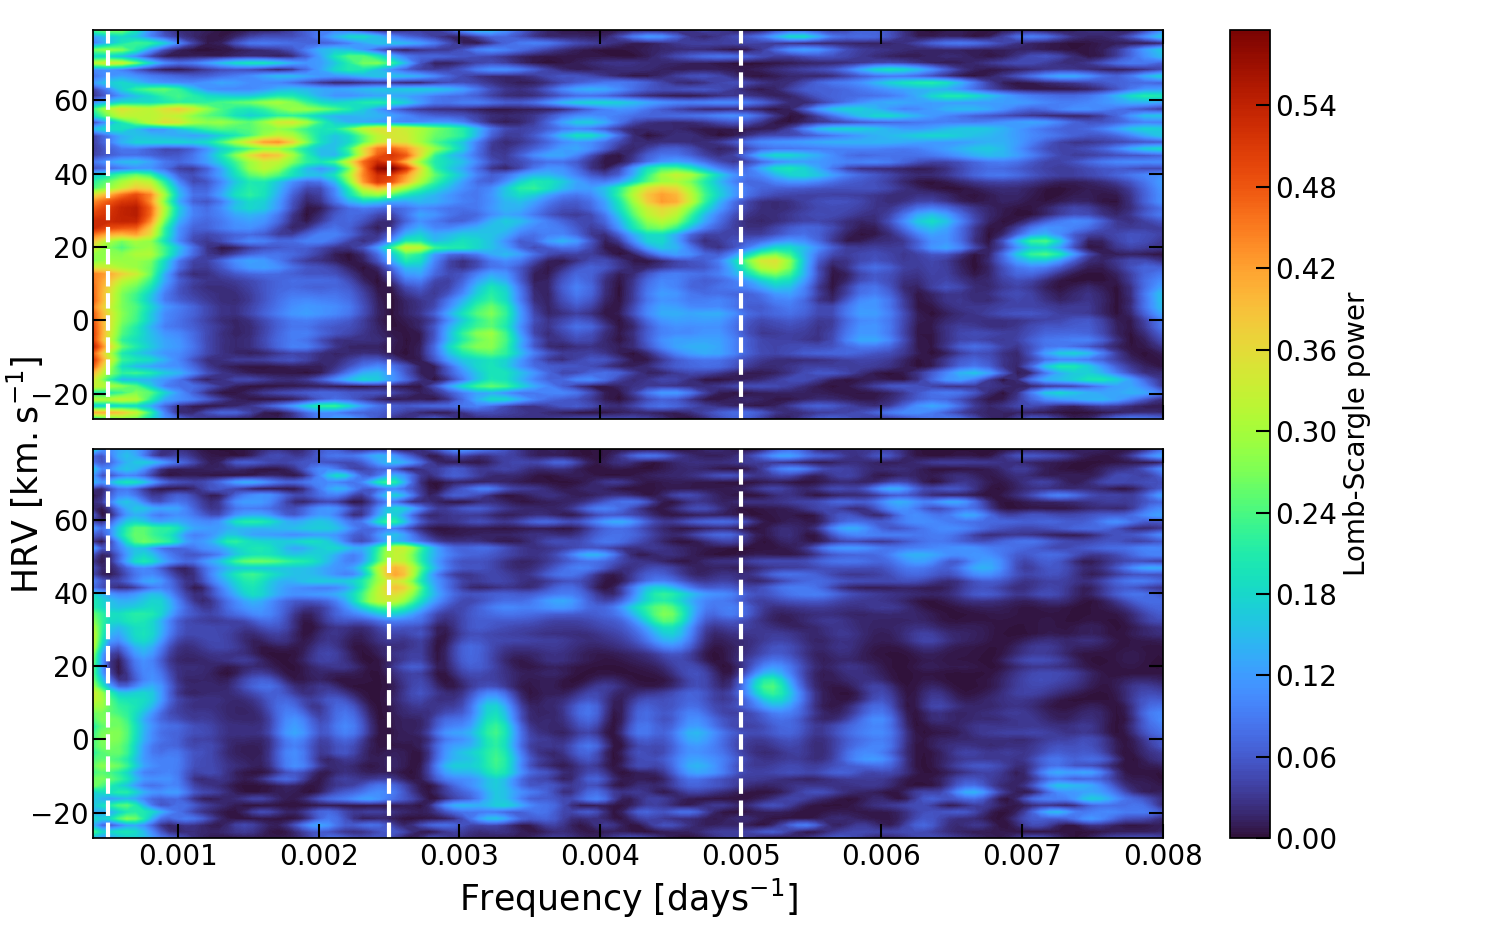
\includegraphics[width=\textwidth]{Lomb-Scargle linear polarization.png}
    \caption{Same as figure \ref{LS intensity}, but for the linear polarization: $\sqrt{\mathrm{Q^2}+\mathrm{U^2}}$.}
    \label{LS linear polarization}
\end{figure*}



\section{Recovering periodicity of Betelgeuse in the LSD profile}

\subsection{Intensity}
Figure \ref{LS intensity} shows the LS periodogram of the LSD of the intensity profile. Interestingly, we recover the LSP at 2000 days, 
located at a HRV of $\sim$ 20 km/s. This periodicity seems to change after the dimming, where it is located at a HRV between 0 and 10 km/s. 
There is also a weaker signal at the fundamental mode, around 400 days. This signal completely disappears after the dimming. It is hard to attribute 
this LS power to a periodicity of Betelgeuse, however it might be a hint that this periodicity has changed after the dimming. Furthermore, our results 
in the intensity profile are consistent with the one from \cite{Mathias2018} who used 2D fourier analysis and found that the dominant period was the LSP. 
We can also see that there is a less stronger signal at 40 km/s in the LSP. We will discuss about it in the next section, but the fact that there is a weak 
signal at 40 km/s, which is the velocity of the star in the heliocentric reference frame, could be a clue to understand the periodicity of Betelgeuse. 
The intensity is sensitive to the whole star, hence the periodogram of the intensity is sensitive to global variation of the star. It is sensitive to 
the timescale on which giant convective cells evolve. It has been observed that some convective cells can live for more than two years. Even though the
LSP is around five years, we can attribute the LSP to the number of convective cells during a given time. 


\subsection{Stokes Q and U}

Figure \ref{LS Q} and \ref{LS U} show the LS periodogram of both stokes Q and U. It is clear that the LS periodogram is completely different 
from the intensity one. We can see a strong signal in fig. \ref{LS Q} around 200 days. Once again, this signal is much more weak after the dimming.
Concerning stokes U in fig. \ref{LS U}, it appears that we only recover the LSP, which once again, is weaker after the great dimming. 
Those periodograms rise a lot of questions: why is the 200 days period only present in stokes Q? Why not in stokes U or intensity? 
We will discuss about those questions in the next question. However, it also appears that stokes Q is not sensitive to the LSP, or to be more precise, 
it is much more sensitive to the 200 days period. From this, we can conclude that stokes Q evolves on a time scale much more closer to the first overtone 
mode than the LSP or even the fundamental mode. Because stokes Q is sensitive only to shorter periods, the variation of stokes Q come from another mechanism 
than the one from intensity. Because the linear polarization in Betelgeuse is due to convective cells, we attribute the signal present in the periodogram 
as the lifetime of convective cells. This is what we observe in the LSD profile of Betelgeuse: from a week to another it does not change that much. 
However, after a few month, the LSD profile of Betelgeuse has completely changed, due to the evolution of convective cells at the surface. 
This would explain the strong signal present at 200 days in stokes Q. 


\subsection{The linear polarization}

Figure \ref{LS linear polarization} shows the LS periodogram of the linear polarization of Betelgeuse: $\sqrt{\mathrm{Q^2+U^2}}$. 
Interestingly, the LS periodogram shows a strong power at 400 days and 2000 days. This signal is much more weaker after the dimming.
While the LSP is already present in the LS of intensity, here we recover the 400 days periodicity, often invoke in the literature. 
Nonetheless, the period is present at a HRV of around 40 km/s. We recall that this velocity is the velocity of the star \cite{LopezAriste2018}. 
Every signal above the velocity of the star is either due to the plasma sinking in Betelgeuse, or plumes of plasma rising above the limb of the star, 
as seen in other red supergiant like $\mu$Cep \citep{LopezAriste2023}. Up to this point, we want to pinpoint the two elements that are a clue 
to understand the variability of Betelgeuse: the 400 days period is present in the linear polarization signal and also at a HRV above 40 km/s.
In any case, from the linear polarization and the intensity profile, we recover the different periods of Betelgeuse.


\section{Convection to explain periodicities}

In the previous section, we have seen that we recover the different period of Betelgeuse from the intensity and linear polarization signal. 
While the nature of the LSP is still in debate, the nature of the lower periods is attributed to pulsation of the atmosphere of Betelgeuse 
(e.g \cite{Kiss2006}). The mechanism behind the pulsation of Betelgeuse is attributed to the $\kappa$-mechanism. In this section, we attempt to 
find an explanation to the 400 days periodicity of Betelgeuse. As mentioned before, the LS periodogram of linear polarization shows a periodicity 
around 400 days. Furthermore, the region where the LS power is high around 40km/s. This wavelength correspond to the red wing of Betelgeuse.
The polarization signal is supposed to stand between -20 and 40km/s. Signal above 40km/s is associated to plasma rising behind the limb of Betelgeuse. 
This mechanism has been observed in the RSG $\mu$Cep and was introduced by \cite{LopezAriste2023} to explain the excess of linear polarization beyond 
the velocity of the star. In $\mu$Cep, the linear polarization signal is very strong and often present, whereas in Betelgeuse, the signal above the 
velocity of the star is less strong. However, because it is present from time to time, the LS periodogram finds this signal above the limb and finds a
periodicity at this wavelength of 40 km/s. Hence, the strong power associated to this wavelength might be due to those convective plumes that are 
rising above the limb from time to time. From this scenario, we can explained the 400 days period in the light curve as follow: from time to time,
Betelgeuse is ejecting plasma in the interstellar medium due to winds. The plasma can be ejected from the hidden face of Betelgeuse. 
It rises so high that we can see the rising plume from the Earth, because the plume rises above the limb of the star. Hence, from Earth, 
the signal associated to this plume appears redshifted compared to the velocity of the star. This plume increases the number of photons that we receive,
leading to an increase of the brightness. After a few weeks or months, the plume falls back to Betelgeuse, desapearing from our point of view, 
leading to a decrease of the brightness of Betelgeuse. This is exactly what we see is the LSD profile of the linear polarization of Betelgeuse: 
from time to time, there is a net signal above 40km/s, which is present for a few weeks, and then disappears. Since this signal is not always present, 
it is found by the LS periodogram as a periodic event. However, it is not periodic at all: because the plumes rise at random moments, sometimes they 
appear every years, sometime more often. This would explain why we only see it before the dimming, after the dimming, this kind of event never happened 
for the moment. Thus, the LS periodogram, at that precise frequency, finds that there is a periodic signal before the dimming, but not after, leading to
a lower LS power at this frequency. Concerning the 200 days period, it is caused by the timescale on which the stokes parameters evolve. For example, the 
LSD profile of stokes Q or U will slightly change if we observe Betelgeuse every two weeks. However, on a longer timescale, for example a few month, 
the LSD profile of stokes Q and U will change a lot. They are directly linked to the dynamics of the surface, hence,  their variation scale the lifetime 
of convective cells. Some convective cells can live up to a few month, leading to this peak in the LS periodogram of stokes Q. As showed by
\cite{LopezAriste2018}, some convective cells can live up to years, explaining also the LSP. One can notice that the peak is not present in stokes U. 
However, if we try to explain the periodicity of Betelgeuse using pulsations, we would see this signal in either stokes U and the linear polarization. 
To summarise what we have done so far: we were able to explain the variability of Betelgeuse by using surface convection only. The convective cells play 
the most important role in the variability of Betelgeuse. Our work does not need pulsation to explain its variability. This does not mean that there are 
no pulsation in Betelgeuse. What we claim is that the most important factor in the variability of Betelgeuse is the timescale on which the convective 
cells evolve. Pulsation could exist on Betelgeuse, but probably on shorter timescale than the one observed. 

\begin{acknowledgements}
    This work was supported by the "Programme National de Physique Stellaire" (PNPS) of CNRS/INSU co-funded by CEA and CNES.
    We acknowledge support from the French National Research Agency (ANR)
    funded project PEPPER (ANR-20-CE31-0002)
    \end{acknowledgements}
    
    \bibliographystyle{aa}
    %\bibliographystyle{aa}
    
    \bibliography{art75}
\end{document}


